% Options for packages loaded elsewhere
\PassOptionsToPackage{unicode}{hyperref}
\PassOptionsToPackage{hyphens}{url}
\PassOptionsToPackage{dvipsnames,svgnames,x11names}{xcolor}
%
\documentclass[
  letterpaper,
  DIV=11,
  numbers=noendperiod]{scrartcl}

\usepackage{amsmath,amssymb}
\usepackage{iftex}
\ifPDFTeX
  \usepackage[T2A]{fontenc}
  \usepackage[utf8]{inputenc}
  \usepackage{textcomp} % provide euro and other symbols
\else % if luatex or xetex
  \usepackage{unicode-math}
  \defaultfontfeatures{Scale=MatchLowercase}
  \defaultfontfeatures[\rmfamily]{Ligatures=TeX,Scale=1}
\fi
\usepackage{lmodern}
\ifPDFTeX\else  
    % xetex/luatex font selection
  \setmainfont[]{CMU Serif}
  \setsansfont[]{CMU Serif}
  \setmonofont[]{CMU Serif}
\fi
% Use upquote if available, for straight quotes in verbatim environments
\IfFileExists{upquote.sty}{\usepackage{upquote}}{}
\IfFileExists{microtype.sty}{% use microtype if available
  \usepackage[]{microtype}
  \UseMicrotypeSet[protrusion]{basicmath} % disable protrusion for tt fonts
}{}
\makeatletter
\@ifundefined{KOMAClassName}{% if non-KOMA class
  \IfFileExists{parskip.sty}{%
    \usepackage{parskip}
  }{% else
    \setlength{\parindent}{0pt}
    \setlength{\parskip}{6pt plus 2pt minus 1pt}}
}{% if KOMA class
  \KOMAoptions{parskip=half}}
\makeatother
\usepackage{xcolor}
\setlength{\emergencystretch}{3em} % prevent overfull lines
\setcounter{secnumdepth}{-\maxdimen} % remove section numbering
% Make \paragraph and \subparagraph free-standing
\ifx\paragraph\undefined\else
  \let\oldparagraph\paragraph
  \renewcommand{\paragraph}[1]{\oldparagraph{#1}\mbox{}}
\fi
\ifx\subparagraph\undefined\else
  \let\oldsubparagraph\subparagraph
  \renewcommand{\subparagraph}[1]{\oldsubparagraph{#1}\mbox{}}
\fi


\providecommand{\tightlist}{%
  \setlength{\itemsep}{0pt}\setlength{\parskip}{0pt}}\usepackage{longtable,booktabs,array}
\usepackage{calc} % for calculating minipage widths
% Correct order of tables after \paragraph or \subparagraph
\usepackage{etoolbox}
\makeatletter
\patchcmd\longtable{\par}{\if@noskipsec\mbox{}\fi\par}{}{}
\makeatother
% Allow footnotes in longtable head/foot
\IfFileExists{footnotehyper.sty}{\usepackage{footnotehyper}}{\usepackage{footnote}}
\makesavenoteenv{longtable}
\usepackage{graphicx}
\makeatletter
\def\maxwidth{\ifdim\Gin@nat@width>\linewidth\linewidth\else\Gin@nat@width\fi}
\def\maxheight{\ifdim\Gin@nat@height>\textheight\textheight\else\Gin@nat@height\fi}
\makeatother
% Scale images if necessary, so that they will not overflow the page
% margins by default, and it is still possible to overwrite the defaults
% using explicit options in \includegraphics[width, height, ...]{}
\setkeys{Gin}{width=\maxwidth,height=\maxheight,keepaspectratio}
% Set default figure placement to htbp
\makeatletter
\def\fps@figure{htbp}
\makeatother

\KOMAoption{captions}{tableheading}
\usepackage[authordate, abbreviate = true, date = year, autocite=inline, backref = true]{biblatex-chicago}
\usepackage{csquotes}
\setlength{\bibhang}{0pt}
\makeatletter
\makeatother
\makeatletter
\makeatother
\makeatletter
\@ifpackageloaded{caption}{}{\usepackage{caption}}
\AtBeginDocument{%
\ifdefined\contentsname
  \renewcommand*\contentsname{Table of contents}
\else
  \newcommand\contentsname{Table of contents}
\fi
\ifdefined\listfigurename
  \renewcommand*\listfigurename{List of Figures}
\else
  \newcommand\listfigurename{List of Figures}
\fi
\ifdefined\listtablename
  \renewcommand*\listtablename{List of Tables}
\else
  \newcommand\listtablename{List of Tables}
\fi
\ifdefined\figurename
  \renewcommand*\figurename{Figure}
\else
  \newcommand\figurename{Figure}
\fi
\ifdefined\tablename
  \renewcommand*\tablename{Table}
\else
  \newcommand\tablename{Table}
\fi
}
\@ifpackageloaded{float}{}{\usepackage{float}}
\floatstyle{ruled}
\@ifundefined{c@chapter}{\newfloat{codelisting}{h}{lop}}{\newfloat{codelisting}{h}{lop}[chapter]}
\floatname{codelisting}{Listing}
\newcommand*\listoflistings{\listof{codelisting}{List of Listings}}
\makeatother
\makeatletter
\@ifpackageloaded{caption}{}{\usepackage{caption}}
\@ifpackageloaded{subcaption}{}{\usepackage{subcaption}}
\makeatother
\makeatletter
\@ifpackageloaded{tcolorbox}{}{\usepackage[skins,breakable]{tcolorbox}}
\makeatother
\makeatletter
\@ifundefined{shadecolor}{\definecolor{shadecolor}{rgb}{.97, .97, .97}}
\makeatother
\makeatletter
\makeatother
\makeatletter
\makeatother
\ifLuaTeX
\usepackage[bidi=basic]{babel}
\else
\usepackage[bidi=default]{babel}
\fi
\babelprovide[main,import]{english}
% get rid of language-specific shorthands (see #6817):
\let\LanguageShortHands\languageshorthands
\def\languageshorthands#1{}
\ifLuaTeX
  \usepackage{selnolig}  % disable illegal ligatures
\fi
\usepackage[]{biblatex}
\usepackage{csquotes}
\IfFileExists{bookmark.sty}{\usepackage{bookmark}}{\usepackage{hyperref}}
\IfFileExists{xurl.sty}{\usepackage{xurl}}{} % add URL line breaks if available
\urlstyle{same} % disable monospaced font for URLs
\hypersetup{
  pdftitle={Student dropout analysis based on previously acquired educational achievements: A case of the University of Portalegre},
  pdfauthor={Izeldeen Nedal Yunis Al Fraijat; Danat Semeneev; Ieva Žube; Pankaj Chattri; Kristaps Eglītis},
  pdflang={en},
  pdfkeywords={AA1, AA2},
  colorlinks=true,
  linkcolor={blue},
  filecolor={Maroon},
  citecolor={Blue},
  urlcolor={Blue},
  pdfcreator={LaTeX via pandoc}}

\title{Student dropout analysis based on previously acquired educational
achievements: A case of the University of Portalegre}
\usepackage{etoolbox}
\makeatletter
\providecommand{\subtitle}[1]{% add subtitle to \maketitle
  \apptocmd{\@title}{\par {\large #1 \par}}{}{}
}
\makeatother
\subtitle{Business Analysis, Business Informatics Ms, Fall 2023.}
\author{Izeldeen Nedal Yunis Al Fraijat \and Danat Semeneev \and Ieva
Žube \and Pankaj Chattri \and Kristaps Eglītis\footnote{Rīga Technical
  University}}
\date{2023-12-11}

\begin{document}
\maketitle
\begin{abstract}
.
\end{abstract}
\ifdefined\Shaded\renewenvironment{Shaded}{\begin{tcolorbox}[interior hidden, sharp corners, boxrule=0pt, enhanced, frame hidden, borderline west={3pt}{0pt}{shadecolor}, breakable]}{\end{tcolorbox}}\fi

\hypertarget{abstract}{%
\subsection{Abstract}\label{abstract}}

In the world of education, the path to success is often visualized as a
linear progression, where students follow a predefined journey from
kindergarten to graduation. However, the reality is far more complex.
Various reasons lead students to choose to deviate from this path. These
students have encountered different challenges, circumstances, or a lack
of proper resources that have led them to drop out of university.

In this dataset provided to us, we will delve deeper into understanding
the reasons why students have dropped out of the university, based on
the data at our disposal. We will leverage our social knowledge to
comprehend the factors that influenced their decision to drop out and
work to prevent such occurrences if the issues are within the
university's purview. Our goal is to offer solutions, support, and the
necessary resources to facilitate students' educational journeys. We
will also use the analysis we've conducted on the dropout students to
learn from their experiences and chart a unique educational pathway with
fewer dropouts.

\hypertarget{introduction}{%
\section{Introduction}\label{introduction}}

Starting from preliminary school we are told that having an education is
very important for your future or that without higher education your job
possibilities are going to be very limited. While primary education is
mandatory, having higher education is not. But why do people actually
take their time and resources to pursue it? Well, according to studies
the most important factor for pursuing higher education is job
acquisition. Some other factors may include increased income in the
existing job, improved work conditions or increased ability for
retirement. All in all they do all tie up to materialistic benefits in
the end. Of course, other, more intrisic factors include seeking for
additional knowledge or self-fulfillment. There are also factors like
meeting new friends, improving social interaction skills or just wanting
to make a difference in the world. Of course factors that cannot be
ignored are social pressure, meaning that having friends that want to
pursue higher education can influence ones own decision or influence of
family members. Pursuing higher edication is good, but what about people
who prematurely end their studies and drop out? What could be the
factors that lead to such a decision? Based on the study and datasets
that we used for our research there are multiple factors that influence
dropping out.

Nevertheless, pursuing higher education and actually getting the degree
has some tangible benefits. According to an OECD -- Education at a
Glance 2019 research paper, \enquote{On average across OECD countries,
adults with a short-cycle tertiary degree earn 20\% more than adults
with upper secondary education. The earnings advantage increases to 44\%
for those with a bachelor's degree and to 91\% for those with a master's
or doctoral degree.} With this in mind, it is important for government
and educational institutions to ensure high level of graduates in
society to ensure economic growth and overall increase in well-being. To
measure the success of this goal, it is important to set KPI's, track
them and make educated conclusions on what needs to be done or is being
done right to reach the goal of higher educated society.

\hypertarget{target-metrics-and-kpi}{%
\subsection{Target Metrics and KPI}\label{target-metrics-and-kpi}}

In this particular case, KPI's will be chosen based on datasets of
Portugese Schools but most likely data can be generalised, atleast for
Europe, as the region and sociodemographics are not so different. Even
though there are many factors that influence the success of graduation,
only factors that can be proven upon by government and educational
institutions will be chosen. 1st KPI chosen is Academic support. Based
on the dataset students who had support had 3x lower dropout rates than
students that didn't have. This means that governments should be
incentivised to allocate a higher amount of budget towards education to
give financial aid and motivate students to complete their studies.

2nd KPI chosen is Institutional improvements. Again, based on datasets,
schools with improvements have 40\% less dropout rate than schools
without. This is something that can be improved by incentivizing
teachers with higher salaries or giving schools more budget to improve
their workstations.

3rd KPI chosen is grades. Datasets tell us that the higher the average
grade, the lower the dropout rate. Usually students that have low grades
are uninterested in the subjects which could be due to having chosen not
the right program for them or that the way lectures and information is
presented is uninteresting or outdated. Either way this can be improved.
Increasing the possibility that the student has chosen the right program
for him can be done by introducing more \enquote{open days} in higher
education institutions and having more upfront information about what
can be expected from programs. The overall lecture performance can be
improved by taking more time to have up-to-date information presented
and teachers having decent motivation of teaching students. This can be
achieved by increasing teacher salaries and institutions having more
control over teachers and information they present to students.

\hypertarget{exploratory-data-analysis}{%
\subsection{Exploratory Data Analysis}\label{exploratory-data-analysis}}

\begin{verbatim}
Marital status                                      int64
Application mode                                    int64
Application order                                   int64
Course                                              int64
Daytime/evening attendance\t                        int64
Previous qualification                              int64
Previous qualification (grade)                    float64
Nacionality                                         int64
Mother's qualification                              int64
Father's qualification                              int64
Mother's occupation                                 int64
Father's occupation                                 int64
Admission grade                                   float64
Displaced                                           int64
Educational special needs                           int64
Debtor                                              int64
Tuition fees up to date                             int64
Gender                                              int64
Scholarship holder                                  int64
Age at enrollment                                   int64
International                                       int64
Curricular units 1st sem (credited)                 int64
Curricular units 1st sem (enrolled)                 int64
Curricular units 1st sem (evaluations)              int64
Curricular units 1st sem (approved)                 int64
Curricular units 1st sem (grade)                  float64
Curricular units 1st sem (without evaluations)      int64
Curricular units 2nd sem (credited)                 int64
Curricular units 2nd sem (enrolled)                 int64
Curricular units 2nd sem (evaluations)              int64
Curricular units 2nd sem (approved)                 int64
Curricular units 2nd sem (grade)                  float64
Curricular units 2nd sem (without evaluations)      int64
Unemployment rate                                 float64
Inflation rate                                    float64
GDP                                               float64
Target                                             object
dtype: object
\end{verbatim}

\begin{verbatim}
Marital status                                    0
Application mode                                  0
Application order                                 0
Course                                            0
Daytime/evening attendance\t                      0
Previous qualification                            0
Previous qualification (grade)                    0
Nacionality                                       0
Mother's qualification                            0
Father's qualification                            0
Mother's occupation                               0
Father's occupation                               0
Admission grade                                   0
Displaced                                         0
Educational special needs                         0
Debtor                                            0
Tuition fees up to date                           0
Gender                                            0
Scholarship holder                                0
Age at enrollment                                 0
International                                     0
Curricular units 1st sem (credited)               0
Curricular units 1st sem (enrolled)               0
Curricular units 1st sem (evaluations)            0
Curricular units 1st sem (approved)               0
Curricular units 1st sem (grade)                  0
Curricular units 1st sem (without evaluations)    0
Curricular units 2nd sem (credited)               0
Curricular units 2nd sem (enrolled)               0
Curricular units 2nd sem (evaluations)            0
Curricular units 2nd sem (approved)               0
Curricular units 2nd sem (grade)                  0
Curricular units 2nd sem (without evaluations)    0
Unemployment rate                                 0
Inflation rate                                    0
GDP                                               0
Target                                            0
dtype: int64
\end{verbatim}

Later on, we get the basic descriptive statistics, shown below.

\begin{longtable}[]{@{}llllllllllllllllllllll@{}}
\toprule\noalign{}
& Marital status & Application mode & Application order & Course &
Daytime/evening attendance & Previous qualification & Previous
qualification (grade) & Nacionality & Mother\textquotesingle s
qualification & Father\textquotesingle s qualification & ... &
Curricular units 1st sem (without evaluations) & Curricular units 2nd
sem (credited) & Curricular units 2nd sem (enrolled) & Curricular units
2nd sem (evaluations) & Curricular units 2nd sem (approved) & Curricular
units 2nd sem (grade) & Curricular units 2nd sem (without evaluations) &
Unemployment rate & Inflation rate & GDP \\
\midrule\noalign{}
\endhead
\bottomrule\noalign{}
\endlastfoot
count & 4424.000000 & 4424.000000 & 4424.000000 & 4424.000000 &
4424.000000 & 4424.000000 & 4424.000000 & 4424.000000 & 4424.000000 &
4424.000000 & ... & 4424.000000 & 4424.000000 & 4424.000000 &
4424.000000 & 4424.000000 & 4424.000000 & 4424.000000 & 4424.000000 &
4424.000000 & 4424.000000 \\
mean & 1.178571 & 18.669078 & 1.727848 & 8856.642631 & 0.890823 &
4.577758 & 132.613314 & 1.873192 & 19.561935 & 22.275316 & ... &
0.137658 & 0.541817 & 6.232143 & 8.063291 & 4.435805 & 10.230206 &
0.150316 & 11.566139 & 1.228029 & 0.001969 \\
std & 0.605747 & 17.484682 & 1.313793 & 2063.566416 & 0.311897 &
10.216592 & 13.188332 & 6.914514 & 15.603186 & 15.343108 & ... &
0.690880 & 1.918546 & 2.195951 & 3.947951 & 3.014764 & 5.210808 &
0.753774 & 2.663850 & 1.382711 & 2.269935 \\
min & 1.000000 & 1.000000 & 0.000000 & 33.000000 & 0.000000 & 1.000000 &
95.000000 & 1.000000 & 1.000000 & 1.000000 & ... & 0.000000 & 0.000000 &
0.000000 & 0.000000 & 0.000000 & 0.000000 & 0.000000 & 7.600000 &
-0.800000 & -4.060000 \\
25\% & 1.000000 & 1.000000 & 1.000000 & 9085.000000 & 1.000000 &
1.000000 & 125.000000 & 1.000000 & 2.000000 & 3.000000 & ... & 0.000000
& 0.000000 & 5.000000 & 6.000000 & 2.000000 & 10.750000 & 0.000000 &
9.400000 & 0.300000 & -1.700000 \\
50\% & 1.000000 & 17.000000 & 1.000000 & 9238.000000 & 1.000000 &
1.000000 & 133.100000 & 1.000000 & 19.000000 & 19.000000 & ... &
0.000000 & 0.000000 & 6.000000 & 8.000000 & 5.000000 & 12.200000 &
0.000000 & 11.100000 & 1.400000 & 0.320000 \\
75\% & 1.000000 & 39.000000 & 2.000000 & 9556.000000 & 1.000000 &
1.000000 & 140.000000 & 1.000000 & 37.000000 & 37.000000 & ... &
0.000000 & 0.000000 & 7.000000 & 10.000000 & 6.000000 & 13.333333 &
0.000000 & 13.900000 & 2.600000 & 1.790000 \\
max & 6.000000 & 57.000000 & 9.000000 & 9991.000000 & 1.000000 &
43.000000 & 190.000000 & 109.000000 & 44.000000 & 44.000000 & ... &
12.000000 & 19.000000 & 23.000000 & 33.000000 & 20.000000 & 18.571429 &
12.000000 & 16.200000 & 3.700000 & 3.510000 \\
\end{longtable}

The students are from multiple countries, but the overwhelming majority
of the students are from Portugal. It would be interesting to see how
the students' admission grade depends on their previous qualification,
particularily because of that many students from abroad are from the
Ultramarine Territories where it's more challenging to get comparable
education.

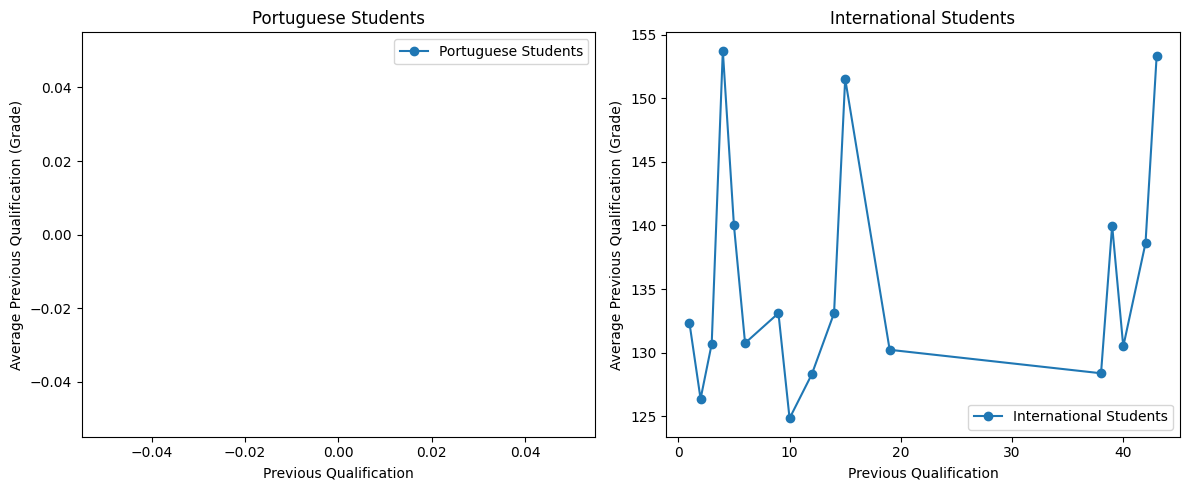
\includegraphics{report_AzadhdhinNedalYunisAlFraijat_files/figure-pdf/cell-7-output-1.png}

Also, there is a drastic imbalance over yet another crucial factor: age.
As it was mentioned previously, students of age are far less ubiquitous,
can have far more incentives to abandon studies and with smaller
potential to apprehension of material. Indeed, this is eloquently
manifested on the next graph.

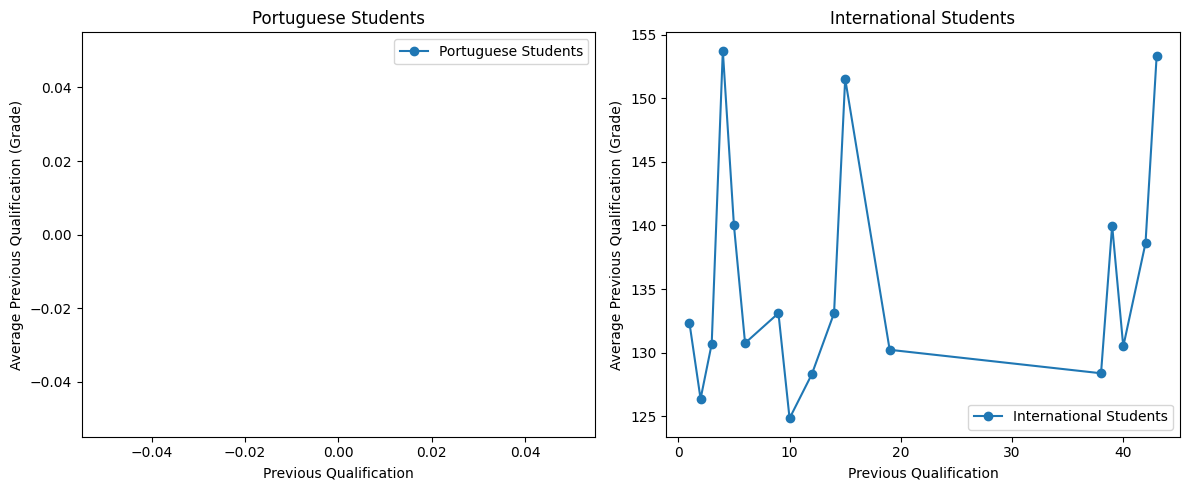
\includegraphics{report_AzadhdhinNedalYunisAlFraijat_files/figure-pdf/cell-8-output-1.png}

Q. v. the sizes of the bins for dropout students differ far less than
the total size for the name of the student.

If the hypothesis about some external factors, The target variable
should be much dependent on previous grades,\\
The datapoint cloud, however, shows that this rule has a lot of
exceptions.

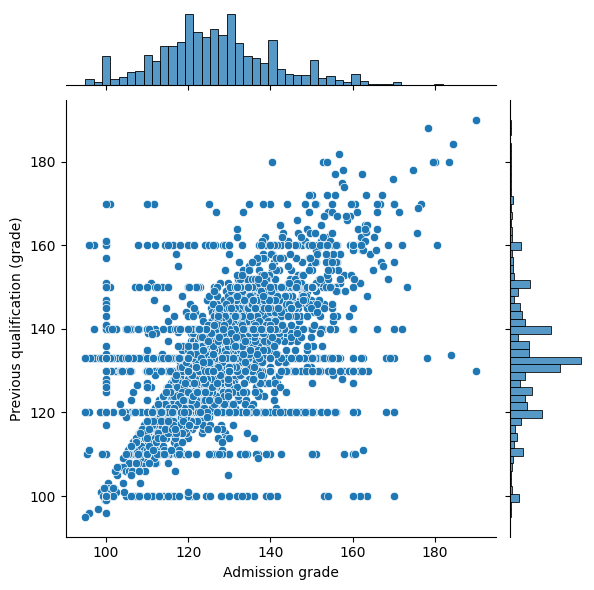
\includegraphics{report_AzadhdhinNedalYunisAlFraijat_files/figure-pdf/cell-10-output-1.png}

We can draw the following observations:

\begin{itemize}
\item
  The \textbf{distribution of admission grades} is roughly normal with
  most students scoring between \textbf{\emph{60 to 80 marks}}.
\item
  The \textbf{distribution of previous qualifications} (grades) is also
  the same with most of them having grades in between \textbf{\emph{12
  and 16}}.
\item
  There is seen a \textbf{positive correlation} between admission grade
  and previous qualification grade indicating students with higher
  previous qualifications tend to have higher admission grades.
\end{itemize}

In the previous graphs, we considered qualitative columns that are more
or less exogenous to the dataset.

However, the majority of columns of this dataset are qualitative and
they do not much fit, so we would opt for analysis of discriminate
groups. This was the visualization for the few quantitative columns,
which shows the natural interconnection between the curricularly accrued
units in the 1st and the 2nd year, which are in turn mostly unrelated to
the admission grade. This is understandable since the grades are
commonly based on the successfulness of the local program and student's
toil, while the students backgrounds are commonly different and this
puts them into inequitable positions when passing the admission exams.

We also consider the impact of scholarships and other compensations in
academic support, which should quench the complications associated with
adaptations in new environment.

\begin{verbatim}
Text(0.5, 1.0, 'Influence of Socioeconomic Factors on Dropout Rates')
\end{verbatim}

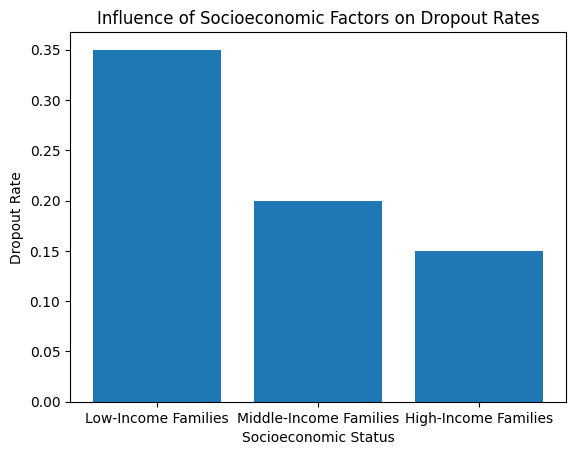
\includegraphics{report_AzadhdhinNedalYunisAlFraijat_files/figure-pdf/cell-11-output-2.png}

\textbf{Observations :}

\begin{itemize}
\tightlist
\item
  Students coming from \emph{low - income families have a higher dropout
  rate} than compared from middle - income and high - income families.
\end{itemize}

Furthermore, not only the pecuniary, but also institutional aspects can
be improved -- and so influence the academic success. Below we
demonstrate how the institutional improvements can influence the
dropout.

\begin{verbatim}
Text(0.5, 1.0, 'Effect of Institutional Improvements on Student Retention')
\end{verbatim}

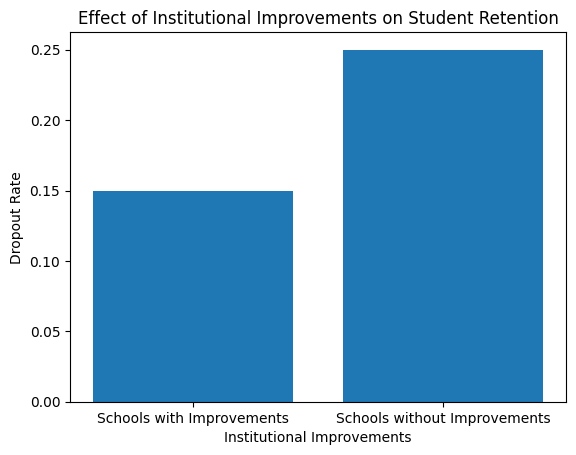
\includegraphics{report_AzadhdhinNedalYunisAlFraijat_files/figure-pdf/cell-12-output-2.png}

\textbf{Observations :}

\begin{itemize}
\tightlist
\item
  Schools having \emph{implemented institutional improvements yeilds a
  significant lowering of the dropout rate} when compared to those
  without.
\end{itemize}

In different studies, it is quite common to compare the academic success
of a student with the academic successes of ttheir parents as this has
both direct and indirect effects , s. a. i. e. both are connected to
welfare, but also it can be that there is another channel of knowledge
transmission to the younger generation.

\begin{verbatim}
Text(0.5, 1.0, "Influence of Mother's Occupation on Dropout Rates")
\end{verbatim}

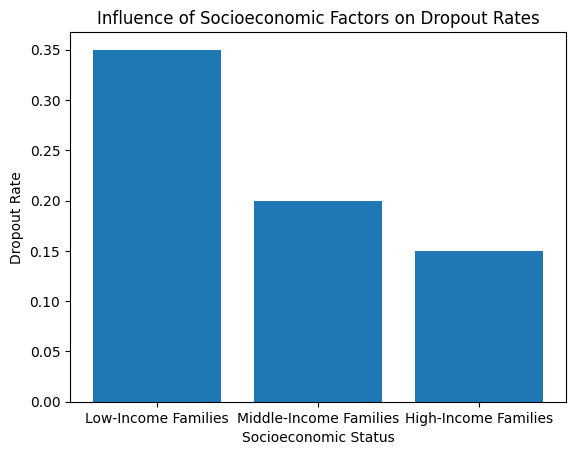
\includegraphics{report_AzadhdhinNedalYunisAlFraijat_files/figure-pdf/cell-13-output-2.png}

\textbf{Observations :}

\begin{itemize}
\item
  The bar chart shows that \emph{Students with mothers in lower-level
  occupations} tend to have higher dropout rates than compared to those
  with mothers in high paying jobs.
\item
  This also may suggest the mother's occupation can influence student
  retention, emphasizing the need for financial support and family
  engagement.
\end{itemize}

\begin{verbatim}
Collecting plotly
  Using cached plotly-5.18.0-py3-none-any.whl (15.6 MB)
Collecting tenacity>=6.2.0
  Using cached tenacity-8.2.3-py3-none-any.whl (24 kB)
Requirement already satisfied: packaging in /Users/romulaperov/.pyenv/versions/3.11.1/lib/python3.11/site-packages (from plotly) (23.2)
Installing collected packages: tenacity, plotly
Successfully installed plotly-5.18.0 tenacity-8.2.3

[notice] A new release of pip available: 22.3.1 -> 23.3.1
[notice] To update, run: pip install --upgrade pip
\end{verbatim}

\begin{verbatim}
ModuleNotFoundError: No module named 'sklearn'
\end{verbatim}

\begin{verbatim}
Collecting pycaret
  Using cached pycaret-3.2.0-py3-none-any.whl (484 kB)
Collecting category-encoders>=2.4.0
  Using cached category_encoders-2.6.3-py2.py3-none-any.whl (81 kB)
Collecting cloudpickle
  Using cached cloudpickle-3.0.0-py3-none-any.whl (20 kB)
Collecting deprecation>=2.1.0
  Using cached deprecation-2.1.0-py2.py3-none-any.whl (11 kB)
Collecting imbalanced-learn>=0.8.1
  Using cached imbalanced_learn-0.11.0-py3-none-any.whl (235 kB)
Collecting importlib-metadata>=4.12.0
  Downloading importlib_metadata-7.0.0-py3-none-any.whl (23 kB)
Requirement already satisfied: ipython>=5.5.0 in /Users/romulaperov/.pyenv/versions/3.11.1/lib/python3.11/site-packages (from pycaret) (8.18.1)
Collecting ipywidgets>=7.6.5
  Using cached ipywidgets-8.1.1-py3-none-any.whl (139 kB)
Collecting jinja2>=1.2
  Using cached Jinja2-3.1.2-py3-none-any.whl (133 kB)
Requirement already satisfied: joblib>=1.2.0 in /Users/romulaperov/.pyenv/versions/3.11.1/lib/python3.11/site-packages (from pycaret) (1.3.2)
Collecting kaleido>=0.2.1
  Using cached kaleido-0.2.1-py2.py3-none-macosx_11_0_arm64.whl (85.8 MB)
Collecting lightgbm>=3.0.0
  Using cached lightgbm-4.1.0.tar.gz (1.7 MB)
  Installing build dependencies ... done
  Getting requirements to build wheel ... done
  Installing backend dependencies ... done
  Preparing metadata (pyproject.toml) ... done
Collecting markupsafe>=2.0.1
  Using cached MarkupSafe-2.1.3-cp311-cp311-macosx_10_9_universal2.whl (17 kB)
Collecting matplotlib<=3.6,>=3.3.0
  Using cached matplotlib-3.6.0-cp311-cp311-macosx_11_0_arm64.whl (7.2 MB)
Collecting nbformat>=4.2.0
  Using cached nbformat-5.9.2-py3-none-any.whl (77 kB)
Collecting numba>=0.55.0
  Using cached numba-0.58.1-cp311-cp311-macosx_11_0_arm64.whl (2.6 MB)
Requirement already satisfied: numpy<1.27,>=1.21 in /Users/romulaperov/.pyenv/versions/3.11.1/lib/python3.11/site-packages (from pycaret) (1.26.2)
Collecting pandas<2.0.0,>=1.3.0
  Using cached pandas-1.5.3-cp311-cp311-macosx_11_0_arm64.whl (10.8 MB)
Collecting plotly-resampler>=0.8.3.1
  Using cached plotly_resampler-0.9.1-py3-none-any.whl (73 kB)
Requirement already satisfied: plotly>=5.0.0 in /Users/romulaperov/.pyenv/versions/3.11.1/lib/python3.11/site-packages (from pycaret) (5.18.0)
Collecting pmdarima!=1.8.1,<3.0.0,>=1.8.0
  Using cached pmdarima-2.0.4-cp311-cp311-macosx_11_0_arm64.whl (628 kB)
Requirement already satisfied: psutil>=5.9.0 in /Users/romulaperov/.pyenv/versions/3.11.1/lib/python3.11/site-packages (from pycaret) (5.9.6)
Collecting pyod>=1.0.8
  Downloading pyod-1.1.2.tar.gz (160 kB)
     ━━━━━━━━━━━━━━━━━━━━━━━━━━━━━━━━━━━━━━━ 160.5/160.5 kB 2.8 MB/s eta 0:00:00a 0:00:01
  Preparing metadata (setup.py) ... done
Collecting requests>=2.27.1
  Using cached requests-2.31.0-py3-none-any.whl (62 kB)
Collecting schemdraw==0.15
  Using cached schemdraw-0.15-py3-none-any.whl (106 kB)
Collecting scikit-learn<1.3.0,>=1.0
  Using cached scikit_learn-1.2.2-cp311-cp311-macosx_12_0_arm64.whl (8.4 MB)
Collecting scikit-plot>=0.3.7
  Using cached scikit_plot-0.3.7-py3-none-any.whl (33 kB)
Collecting scipy~=1.10.1
  Using cached scipy-1.10.1-cp311-cp311-macosx_12_0_arm64.whl (28.7 MB)
Collecting sktime!=0.17.1,!=0.17.2,!=0.18.0,<0.22.0,>=0.16.1
  Using cached sktime-0.21.1-py3-none-any.whl (17.1 MB)
Collecting statsmodels>=0.12.1
  Using cached statsmodels-0.14.0-cp311-cp311-macosx_11_0_arm64.whl (9.4 MB)
Collecting tbats>=1.1.3
  Using cached tbats-1.1.3-py3-none-any.whl (44 kB)
Collecting tqdm>=4.62.0
  Using cached tqdm-4.66.1-py3-none-any.whl (78 kB)
Collecting xxhash
  Using cached xxhash-3.4.1-cp311-cp311-macosx_11_0_arm64.whl (30 kB)
Collecting yellowbrick>=1.4
  Using cached yellowbrick-1.5-py3-none-any.whl (282 kB)
Collecting wurlitzer
  Using cached wurlitzer-3.0.3-py3-none-any.whl (7.3 kB)
Collecting patsy>=0.5.1
  Downloading patsy-0.5.4-py2.py3-none-any.whl (233 kB)
     ━━━━━━━━━━━━━━━━━━━━━━━━━━━━━━━━━━━━━━━ 233.9/233.9 kB 2.4 MB/s eta 0:00:00a 0:00:01
Requirement already satisfied: packaging in /Users/romulaperov/.pyenv/versions/3.11.1/lib/python3.11/site-packages (from deprecation>=2.1.0->pycaret) (23.2)
Requirement already satisfied: threadpoolctl>=2.0.0 in /Users/romulaperov/.pyenv/versions/3.11.1/lib/python3.11/site-packages (from imbalanced-learn>=0.8.1->pycaret) (3.2.0)
Collecting zipp>=0.5
  Using cached zipp-3.17.0-py3-none-any.whl (7.4 kB)
Requirement already satisfied: decorator in /Users/romulaperov/.pyenv/versions/3.11.1/lib/python3.11/site-packages (from ipython>=5.5.0->pycaret) (5.1.1)
Requirement already satisfied: jedi>=0.16 in /Users/romulaperov/.pyenv/versions/3.11.1/lib/python3.11/site-packages (from ipython>=5.5.0->pycaret) (0.19.1)
Requirement already satisfied: matplotlib-inline in /Users/romulaperov/.pyenv/versions/3.11.1/lib/python3.11/site-packages (from ipython>=5.5.0->pycaret) (0.1.6)
Requirement already satisfied: prompt-toolkit<3.1.0,>=3.0.41 in /Users/romulaperov/.pyenv/versions/3.11.1/lib/python3.11/site-packages (from ipython>=5.5.0->pycaret) (3.0.41)
Requirement already satisfied: pygments>=2.4.0 in /Users/romulaperov/.pyenv/versions/3.11.1/lib/python3.11/site-packages (from ipython>=5.5.0->pycaret) (2.17.2)
Requirement already satisfied: stack-data in /Users/romulaperov/.pyenv/versions/3.11.1/lib/python3.11/site-packages (from ipython>=5.5.0->pycaret) (0.6.3)
Requirement already satisfied: traitlets>=5 in /Users/romulaperov/.pyenv/versions/3.11.1/lib/python3.11/site-packages (from ipython>=5.5.0->pycaret) (5.14.0)
Requirement already satisfied: pexpect>4.3 in /Users/romulaperov/.pyenv/versions/3.11.1/lib/python3.11/site-packages (from ipython>=5.5.0->pycaret) (4.9.0)
Requirement already satisfied: comm>=0.1.3 in /Users/romulaperov/.pyenv/versions/3.11.1/lib/python3.11/site-packages (from ipywidgets>=7.6.5->pycaret) (0.2.0)
Collecting widgetsnbextension~=4.0.9
  Using cached widgetsnbextension-4.0.9-py3-none-any.whl (2.3 MB)
Collecting jupyterlab-widgets~=3.0.9
  Using cached jupyterlab_widgets-3.0.9-py3-none-any.whl (214 kB)
Requirement already satisfied: contourpy>=1.0.1 in /Users/romulaperov/.pyenv/versions/3.11.1/lib/python3.11/site-packages (from matplotlib<=3.6,>=3.3.0->pycaret) (1.2.0)
Requirement already satisfied: cycler>=0.10 in /Users/romulaperov/.pyenv/versions/3.11.1/lib/python3.11/site-packages (from matplotlib<=3.6,>=3.3.0->pycaret) (0.12.1)
Requirement already satisfied: fonttools>=4.22.0 in /Users/romulaperov/.pyenv/versions/3.11.1/lib/python3.11/site-packages (from matplotlib<=3.6,>=3.3.0->pycaret) (4.46.0)
Requirement already satisfied: kiwisolver>=1.0.1 in /Users/romulaperov/.pyenv/versions/3.11.1/lib/python3.11/site-packages (from matplotlib<=3.6,>=3.3.0->pycaret) (1.4.5)
Requirement already satisfied: pillow>=6.2.0 in /Users/romulaperov/.pyenv/versions/3.11.1/lib/python3.11/site-packages (from matplotlib<=3.6,>=3.3.0->pycaret) (10.1.0)
Requirement already satisfied: pyparsing>=2.2.1 in /Users/romulaperov/.pyenv/versions/3.11.1/lib/python3.11/site-packages (from matplotlib<=3.6,>=3.3.0->pycaret) (3.1.1)
Requirement already satisfied: python-dateutil>=2.7 in /Users/romulaperov/.pyenv/versions/3.11.1/lib/python3.11/site-packages (from matplotlib<=3.6,>=3.3.0->pycaret) (2.8.2)
Collecting fastjsonschema
  Downloading fastjsonschema-2.19.0-py3-none-any.whl (23 kB)
Collecting jsonschema>=2.6
  Using cached jsonschema-4.20.0-py3-none-any.whl (84 kB)
Requirement already satisfied: jupyter-core in /Users/romulaperov/.pyenv/versions/3.11.1/lib/python3.11/site-packages (from nbformat>=4.2.0->pycaret) (5.5.0)
Collecting llvmlite<0.42,>=0.41.0dev0
  Using cached llvmlite-0.41.1-cp311-cp311-macosx_11_0_arm64.whl (28.8 MB)
Requirement already satisfied: pytz>=2020.1 in /Users/romulaperov/.pyenv/versions/3.11.1/lib/python3.11/site-packages (from pandas<2.0.0,>=1.3.0->pycaret) (2023.3.post1)
Requirement already satisfied: tenacity>=6.2.0 in /Users/romulaperov/.pyenv/versions/3.11.1/lib/python3.11/site-packages (from plotly>=5.0.0->pycaret) (8.2.3)
Collecting dash<3.0.0,>=2.11.0
  Downloading dash-2.14.2-py3-none-any.whl (10.2 MB)
     ━━━━━━━━━━━━━━━━━━━━━━━━━━━━━━━━━━━━━━━━ 10.2/10.2 MB 5.1 MB/s eta 0:00:0000:010:01
Collecting orjson<4.0.0,>=3.8.0
  Using cached orjson-3.9.10-cp311-cp311-macosx_10_15_x86_64.macosx_11_0_arm64.macosx_10_15_universal2.whl (242 kB)
Collecting trace-updater>=0.0.8
  Using cached trace_updater-0.0.9.1-py3-none-any.whl (185 kB)
Collecting tsdownsample==0.1.2
  Using cached tsdownsample-0.1.2-cp311-cp311-macosx_11_0_arm64.whl (1.2 MB)
Collecting Cython!=0.29.18,!=0.29.31,>=0.29
  Downloading Cython-3.0.6-py2.py3-none-any.whl (1.2 MB)
     ━━━━━━━━━━━━━━━━━━━━━━━━━━━━━━━━━━━━━━━━ 1.2/1.2 MB 5.0 MB/s eta 0:00:00a 0:00:01
Collecting urllib3
  Using cached urllib3-2.1.0-py3-none-any.whl (104 kB)
Requirement already satisfied: setuptools!=50.0.0,>=38.6.0 in /Users/romulaperov/.pyenv/versions/3.11.1/lib/python3.11/site-packages (from pmdarima!=1.8.1,<3.0.0,>=1.8.0->pycaret) (65.5.0)
Requirement already satisfied: six in /Users/romulaperov/.pyenv/versions/3.11.1/lib/python3.11/site-packages (from pyod>=1.0.8->pycaret) (1.16.0)
Collecting charset-normalizer<4,>=2
  Using cached charset_normalizer-3.3.2-cp311-cp311-macosx_11_0_arm64.whl (118 kB)
Collecting idna<4,>=2.5
  Using cached idna-3.6-py3-none-any.whl (61 kB)
Collecting certifi>=2017.4.17
  Using cached certifi-2023.11.17-py3-none-any.whl (162 kB)
Collecting deprecated>=1.2.13
  Using cached Deprecated-1.2.14-py2.py3-none-any.whl (9.6 kB)
Collecting numpy<1.27,>=1.21
  Using cached numpy-1.25.2-cp311-cp311-macosx_11_0_arm64.whl (14.0 MB)
Collecting scikit-base<0.6.0
  Using cached scikit_base-0.5.2-py3-none-any.whl (118 kB)
Collecting Flask<3.1,>=1.0.4
  Using cached flask-3.0.0-py3-none-any.whl (99 kB)
Collecting Werkzeug<3.1
  Using cached werkzeug-3.0.1-py3-none-any.whl (226 kB)
Collecting dash-html-components==2.0.0
  Using cached dash_html_components-2.0.0-py3-none-any.whl (4.1 kB)
Collecting dash-core-components==2.0.0
  Using cached dash_core_components-2.0.0-py3-none-any.whl (3.8 kB)
Collecting dash-table==5.0.0
  Using cached dash_table-5.0.0-py3-none-any.whl (3.9 kB)
Collecting typing-extensions>=4.1.1
  Using cached typing_extensions-4.9.0-py3-none-any.whl (32 kB)
Collecting retrying
  Using cached retrying-1.3.4-py3-none-any.whl (11 kB)
Collecting ansi2html
  Using cached ansi2html-1.8.0-py3-none-any.whl (16 kB)
Requirement already satisfied: nest-asyncio in /Users/romulaperov/.pyenv/versions/3.11.1/lib/python3.11/site-packages (from dash<3.0.0,>=2.11.0->plotly-resampler>=0.8.3.1->pycaret) (1.5.8)
Collecting wrapt<2,>=1.10
  Using cached wrapt-1.16.0-cp311-cp311-macosx_11_0_arm64.whl (38 kB)
Requirement already satisfied: parso<0.9.0,>=0.8.3 in /Users/romulaperov/.pyenv/versions/3.11.1/lib/python3.11/site-packages (from jedi>=0.16->ipython>=5.5.0->pycaret) (0.8.3)
Collecting attrs>=22.2.0
  Using cached attrs-23.1.0-py3-none-any.whl (61 kB)
Collecting jsonschema-specifications>=2023.03.6
  Using cached jsonschema_specifications-2023.11.2-py3-none-any.whl (17 kB)
Collecting referencing>=0.28.4
  Downloading referencing-0.32.0-py3-none-any.whl (26 kB)
Collecting rpds-py>=0.7.1
  Using cached rpds_py-0.13.2-cp311-cp311-macosx_11_0_arm64.whl (327 kB)
Requirement already satisfied: ptyprocess>=0.5 in /Users/romulaperov/.pyenv/versions/3.11.1/lib/python3.11/site-packages (from pexpect>4.3->ipython>=5.5.0->pycaret) (0.7.0)
Requirement already satisfied: wcwidth in /Users/romulaperov/.pyenv/versions/3.11.1/lib/python3.11/site-packages (from prompt-toolkit<3.1.0,>=3.0.41->ipython>=5.5.0->pycaret) (0.2.12)
Requirement already satisfied: platformdirs>=2.5 in /Users/romulaperov/.pyenv/versions/3.11.1/lib/python3.11/site-packages (from jupyter-core->nbformat>=4.2.0->pycaret) (4.1.0)
Requirement already satisfied: executing>=1.2.0 in /Users/romulaperov/.pyenv/versions/3.11.1/lib/python3.11/site-packages (from stack-data->ipython>=5.5.0->pycaret) (2.0.1)
Requirement already satisfied: asttokens>=2.1.0 in /Users/romulaperov/.pyenv/versions/3.11.1/lib/python3.11/site-packages (from stack-data->ipython>=5.5.0->pycaret) (2.4.1)
Requirement already satisfied: pure-eval in /Users/romulaperov/.pyenv/versions/3.11.1/lib/python3.11/site-packages (from stack-data->ipython>=5.5.0->pycaret) (0.2.2)
Collecting itsdangerous>=2.1.2
  Using cached itsdangerous-2.1.2-py3-none-any.whl (15 kB)
Collecting click>=8.1.3
  Using cached click-8.1.7-py3-none-any.whl (97 kB)
Collecting blinker>=1.6.2
  Using cached blinker-1.7.0-py3-none-any.whl (13 kB)
Building wheels for collected packages: lightgbm
  Building wheel for lightgbm (pyproject.toml) ... done
  Created wheel for lightgbm: filename=lightgbm-4.1.0-py3-none-macosx_13_0_arm64.whl size=1318268 sha256=2e2759bceb44eb685bf7f0bfed59bd241c02f81e758b9c05e233e1e9a6d80602
  Stored in directory: /Users/romulaperov/Library/Caches/pip/wheels/e4/35/af/aa7313e7daa097f9344c68556c7601715c73d52cabc8d2e500
Successfully built lightgbm
Installing collected packages: trace-updater, kaleido, fastjsonschema, dash-table, dash-html-components, dash-core-components, zipp, xxhash, wurlitzer, wrapt, widgetsnbextension, urllib3, typing-extensions, tqdm, scikit-base, schemdraw, rpds-py, retrying, orjson, numpy, markupsafe, llvmlite, jupyterlab-widgets, itsdangerous, idna, deprecation, Cython, cloudpickle, click, charset-normalizer, certifi, blinker, attrs, ansi2html, Werkzeug, tsdownsample, scipy, requests, referencing, patsy, pandas, numba, jinja2, importlib-metadata, deprecated, statsmodels, scikit-learn, matplotlib, lightgbm, jsonschema-specifications, Flask, yellowbrick, sktime, scikit-plot, pyod, pmdarima, jsonschema, ipywidgets, imbalanced-learn, dash, category-encoders, tbats, plotly-resampler, nbformat, pycaret
  Attempting uninstall: numpy
    Found existing installation: numpy 1.26.2
    Uninstalling numpy-1.26.2:
      Successfully uninstalled numpy-1.26.2
  Attempting uninstall: scipy
    Found existing installation: scipy 1.11.4
    Uninstalling scipy-1.11.4:
      Successfully uninstalled scipy-1.11.4
  Attempting uninstall: pandas
    Found existing installation: pandas 2.1.4
    Uninstalling pandas-2.1.4:
      Successfully uninstalled pandas-2.1.4
  Attempting uninstall: scikit-learn
    Found existing installation: scikit-learn 1.3.2
    Uninstalling scikit-learn-1.3.2:
      Successfully uninstalled scikit-learn-1.3.2
  Attempting uninstall: matplotlib
    Found existing installation: matplotlib 3.8.2
    Uninstalling matplotlib-3.8.2:
      Successfully uninstalled matplotlib-3.8.2
  DEPRECATION: pyod is being installed using the legacy 'setup.py install' method, because it does not have a 'pyproject.toml' and the 'wheel' package is not installed. pip 23.1 will enforce this behaviour change. A possible replacement is to enable the '--use-pep517' option. Discussion can be found at https://github.com/pypa/pip/issues/8559
  Running setup.py install for pyod ... done
Successfully installed Cython-3.0.6 Flask-3.0.0 Werkzeug-3.0.1 ansi2html-1.8.0 attrs-23.1.0 blinker-1.7.0 category-encoders-2.6.3 certifi-2023.11.17 charset-normalizer-3.3.2 click-8.1.7 cloudpickle-3.0.0 dash-2.14.2 dash-core-components-2.0.0 dash-html-components-2.0.0 dash-table-5.0.0 deprecated-1.2.14 deprecation-2.1.0 fastjsonschema-2.19.0 idna-3.6 imbalanced-learn-0.11.0 importlib-metadata-7.0.0 ipywidgets-8.1.1 itsdangerous-2.1.2 jinja2-3.1.2 jsonschema-4.20.0 jsonschema-specifications-2023.11.2 jupyterlab-widgets-3.0.9 kaleido-0.2.1 lightgbm-4.1.0 llvmlite-0.41.1 markupsafe-2.1.3 matplotlib-3.6.0 nbformat-5.9.2 numba-0.58.1 numpy-1.25.2 orjson-3.9.10 pandas-1.5.3 patsy-0.5.4 plotly-resampler-0.9.1 pmdarima-2.0.4 pycaret-3.2.0 pyod-1.1.2 referencing-0.32.0 requests-2.31.0 retrying-1.3.4 rpds-py-0.13.2 schemdraw-0.15 scikit-base-0.5.2 scikit-learn-1.2.2 scikit-plot-0.3.7 scipy-1.10.1 sktime-0.21.1 statsmodels-0.14.0 tbats-1.1.3 tqdm-4.66.1 trace-updater-0.0.9.1 tsdownsample-0.1.2 typing-extensions-4.9.0 urllib3-2.1.0 widgetsnbextension-4.0.9 wrapt-1.16.0 wurlitzer-3.0.3 xxhash-3.4.1 yellowbrick-1.5 zipp-3.17.0

[notice] A new release of pip available: 22.3.1 -> 23.3.1
[notice] To update, run: pip install --upgrade pip
\end{verbatim}

In the remaining part, we examine the correlations of endogenous
variables. This does not give a scoop about the source of causation and
is not a good predictor, but exhibits an analysis of autocorrelation
inside the quasi-temporal data.

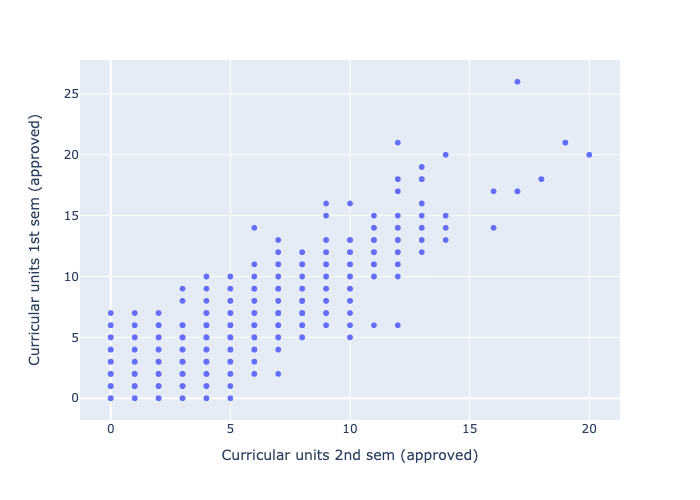
\includegraphics{report_AzadhdhinNedalYunisAlFraijat_files/figure-pdf/cell-33-output-1.png}

We can see that the points for the 1st semester and 2nd semester are
correlated which shows that are one's marks are primary drivers of
success and exhibit sizeable correlations

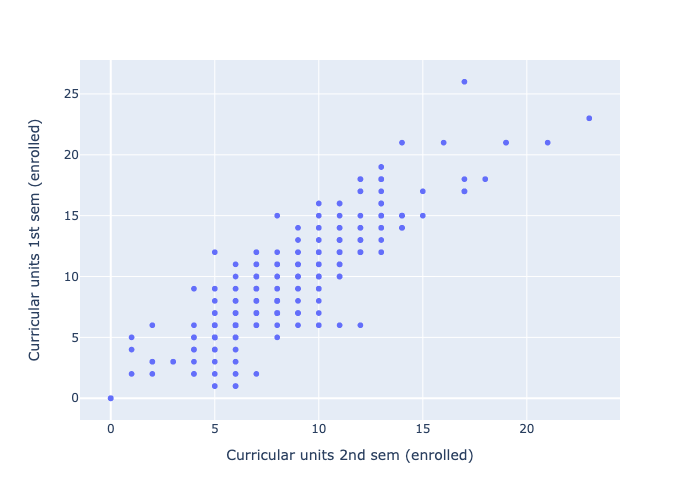
\includegraphics{report_AzadhdhinNedalYunisAlFraijat_files/figure-pdf/cell-34-output-1.png}

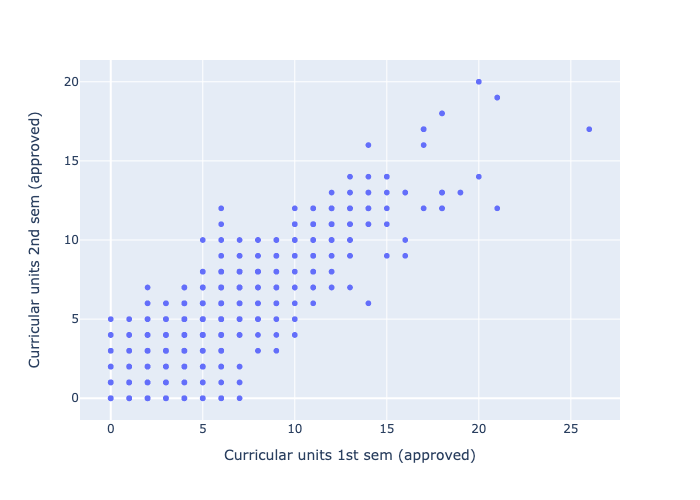
\includegraphics{report_AzadhdhinNedalYunisAlFraijat_files/figure-pdf/cell-35-output-1.png}

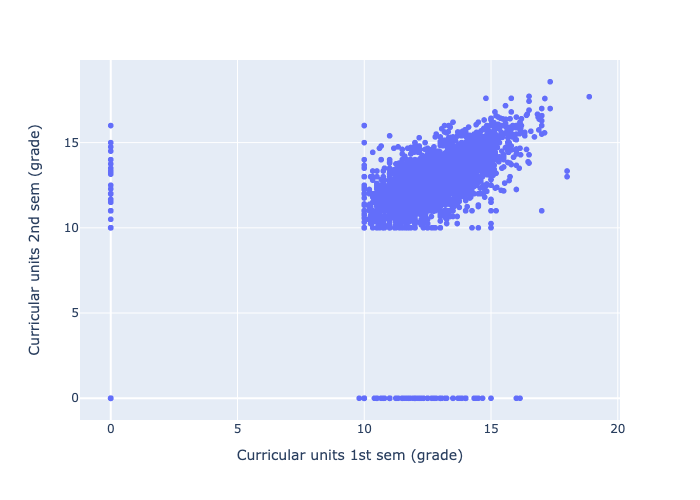
\includegraphics{report_AzadhdhinNedalYunisAlFraijat_files/figure-pdf/cell-36-output-1.png}

\hypertarget{conclusion}{%
\subsection{\texorpdfstring{\textbf{Conclusion}}{Conclusion}}\label{conclusion}}

\begin{quote}
With this analysis, we have some valuable insights some crucial factors
like Academic support, socioeconomic factors, previous qualifications,
and others play a significant role in student retention.
\end{quote}

\begin{quote}
We could work with parents to encourage and support their children's
education. Additionally, We could provide financial assistance to those
who are struggling to pay.
\end{quote}

\begin{quote}
Addressing these factors carefully can effectively lead to dropout rates
reduction and improve overall student outcomes
\end{quote}


\printbibliography


\end{document}
